\documentclass{article}

\usepackage[a4paper,left=2.5cm,right=2.5cm,top=2.5cm,bottom=2.5cm]{geometry}
\usepackage[bahasa]{babel}

\usepackage{lipsum}
\usepackage{graphicx}
\usepackage{hyperref}
% \usepackage{biblatex}
% \addbibresource{main.bib}
\usepackage{apacite}
\usepackage{longtable}
% \usepackage[backend=biber,style=apa,citestyle=apa,sorting=ynt]{biblatex}
% \addbibresource{main.bib}
\usepackage{usebib}
\usepackage{indentfirst}
\bibinput{main}
\graphicspath{ {./images/} }
\title{}

\begin{document}
\begin{center}
    Tugas SIM dan Perencanaan Strategis SI/TI\\
    Balanced Scorecard\\
    62/MMSI/SIB\\
    Ilman Samhabib 91122010\\
    Tri Lestari 91122021\\	
\end{center}
\subsection*{Abstrak}



\emph{Balanced Scorecard} (BSC) memiliki peran penting dalam perencanaan dan perusahaan dengan mengintegrasikan empat perspektif utama. Di sini akan digambarkan pentingnya BSC dalam mengarahkan arah perusahaan, mengukur kinerja, dan mengidentifikasi perbaikan yang perlu. Review ini juga akan mengulas berbagai kegunaan BSC.
\subsection*{Pendahuluan}
\emph{Balanced Scorecard} (BSC) adalah sebuah kerangka yng digunakan dalam proses manajemen untuk mengkomunikasikan apa yang ingin dicapai, dan juga dalam proses pengukuran dan pengawasan pencapaian sebuag target strategis. Sehingga dapat dijadikan pedoman dalam kegiatan bisnis/proses organisasi, seperti dalam menentukan  prioritas proyek, layanan ataupun produk  yang harus didahulukan. BSC juga memfasilitasi pengambilan keputusan yang informatif dengan menyediakan pandangan yang seimbang antara tujuan jangka pendek dan jangka panjang. BSC bersifat fleksibel dalam penentuan prespektif dan dapat digunakan untuk mencatat Indikator Performa Kunci (KPI) tertentu yang ditentukan ataupun disesuaikan dengan kegiatan organisasi. BSC dalam penggunaanya seringkali dilakukan dengan ,memonitor melalui 4 prespektif yaitu  keuangan, pelanggan, proses internal, dan pembelajaran dan pertumbuhan organisasi, di mana akan ditentukan terget dalam keempat hal tersebut dan dibandingkan pencapaian saat ini dengan menngunakan KPI tertentu. 

BSC ataupun sesuatu yang mirip denganya  telah digunakan jauh sejak 1987 \cite{BSCAnalogBibEntry2023Jun} pada perusahaan Analog Devices, dalam menyelaraskan proses bisnisnya dengan perencanaan jangka panjang dan kebutuhan Stakeholder. 
\begin{figure}[htbp]
    \centering
    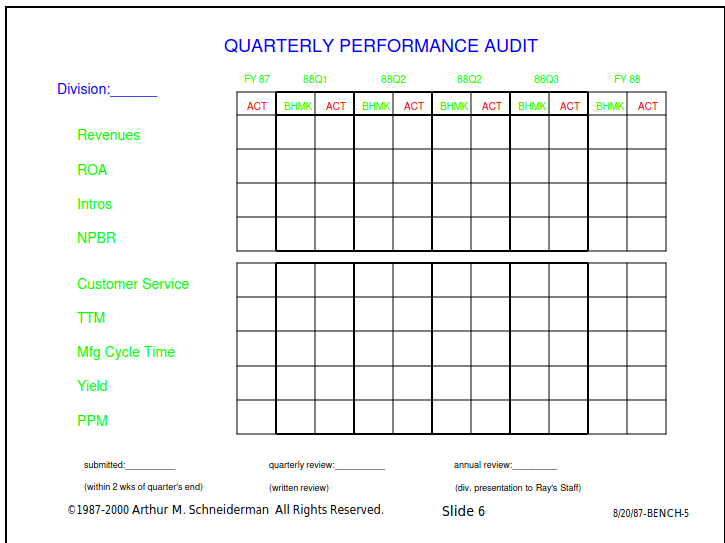
\includegraphics[width=0.8\textwidth]{balanced-scorecard-1987}
    \caption{Versi awal balanced scorecard pada \emph{Analog Devices}}
    \label{fig:my_image}
  \end{figure}\\

Penggunaan BSC telah dilakukan dalam sebuah publikasi artikel pada  tahun 1999. \cite{Talbot1999PublicP} menerapkan  Balanced Scorecard (BSC) untuk mengkaji kinerja dalam konteks pemerintahan, sebagian besar negara anggota organisasi ekonomi kooperatif (OECD). Talbot menggambarkan pentingnya BSC dalam mengarahkan upaya perusahaan, mengukur kinerja secara komprehensif, dan mengidentifikasi peluang perbaikan. Artikel tersebut mengemukakan bahwa konsep kinerja dan model holistik seperti BSC telah berkembang dalam sektor swasta, namun terdapat perbedaan penting antara 'kinerja' di sektor swasta dan sektor publik. Talbot kemudian mengusulkan pendekatan yang relevan, yakni Public Service Excellence Model, untuk meningkatkan kinerja layanan publik. Penelitian ini memberikan wawasan berharga bagi praktisi dan pengambil keputusan dalam konteks kinerja organisasi publik.

Dalam upaya untuk mengatasi kekurangan sistem pengukuran kinerja tradisional, \cite{Kaplan2015TheBS} mengembangkan BSC (Balanced Scorecard). BSC merupakan sebuah sistem pengukuran kinerja baru yang dirancang untuk memberikan pandangan yang komprehensif dari berbagai perspektif perusahaan. Sistem ini mencakup pengukuran keuangan yang memberikan informasi tentang hasil dari tindakan yang sudah dilakukan, serta tiga set pengukuran operasional yang terkait dengan kepuasan pelanggan, proses internal, dan kemampuan belajar dan meningkatkan kinerja organisasi di masa depan. BSC memungkinkan manajer untuk menerjemahkan strategi perusahaan menjadi tujuan yang spesifik dan pengukuran yang relevan, sehingga membantu dalam mengarahkan upaya organisasi secara terkoordinasi. Sebagai contoh, perusahaan Electronic Circuits Inc. berhasil menggunakan BSC untuk mengidentifikasi tujuan kinerja pelanggan dan mengukurnya melalui inisiatif peluncuran produk yang lebih cepat, peningkatan kepuasan pelanggan, kemitraan strategis, dan pengembangan produk inovatif yang sesuai dengan kebutuhan pelanggan.


 
\subsection*{Penelitian Terkini}

\cite{Qiu2020} mengemukakan bahwa manajemen kinerja tradisional yang berbasis indikator keuangan dan kebutuhan akan penerapan teori Balanced Scorecard dalam manajemen kinerja. Model tradisional dibandingkan dengan teori Balanced Scorecard untuk menunjukkan keterbatasannya. Solusinya adalah adopsi teori Balanced Scorecard sebagai kerangka manajemen kinerja. Melalui analisis Alibaba Group sebagai studi kasus BSC, penerapan teori Balanced Scorecard telah berkontribusi pada pertumbuhan dan keunggulan Alibaba Group dalam sistem manajemen kinerja dibandingkan dengan perusahaan e-commerce lainnya. Ini mengimplikasikan bahwa perusahaan lain sebaiknya mempertimbangkan mengadopsi pendekatan Balanced Scorecard dalam manajemen kinerja dalam konteks perkembangan pesat ekonomi internet. Dengan BSC \cite{Qiu2020} menemukan  bahwa Alibaba Group menunjukkan performa yang kuat dalam dimensi keuangan dan pelanggan pada Balanced Scorecard (BSC). Namun, terdapat ruang untuk peningkatan pada dimensi pembelajaran dan pertumbuhan. Perusahaan pun perlu mengatasi masalah pergantian karyawan dan menerapkan strategi untuk membangun budaya pembelajaran yang lebih kuat. Membangun kekuatan tenaga kerja yang solid sangat penting bagi perkembangan Alibaba Group sebagai pemimpin di industri internet.

\cite{Ali2021TheBS} meneliti pengaruh berbagai aspek dari balanced scorecard (proses internal, kapasitas organisasi, dan pelanggan) terhadap mekanisme strategis dalam sektor perbankan. \cite{Ali2021TheBS} melakukan analisis regresi terhadap data yang dikumpulkan dari 128 partisipan,hasilnya adalah dimensi proses internal, kapasitas organisasi, dan pelanggan dalam balanced scorecard memiliki pengaruh positif signifikan terhadap mekanisme strategis pada tingkat signifikansi 5\%. Selain itu, insentif nonfinansial memiliki dampak yang lebih baik terhadap kesuksesan karyawan karena mendorong kesadaran akan lingkungan. \cite{Ali2021TheBS} mengusulkan integrasi inisiatif nonfinansial melengkapi inisiatif finansial untuk meningkatkan proses internal perusahaan. Disarankan juga untuk mengimplementasikan langkah-langkah terkait pengelolaan limbah dan pemanfaatan sumber daya spesifik untuk mendorong perubahan berkelanjutan. Selain itu, penelitian ini menekankan pentingnya melihat pembelajaran dan pengembangan sebagai proses yang berkelanjutan daripada operasi musiman.

\cite{Frederico2020PerformanceMF} teleh meneliti tentang modifikasi BSC untuk memenuhi kebuthuhan industri 4.0, dengan memadukan Lima dimensi utama terkait Industry 4.0 dengan BSC, seperti yang terlihat pada gambar 2. Ini perlu karena  beberapa perbedaan mendasar yang dibawa industri 4.0 contohnya seperti, dimensi baru seperti kemampuan teknologi dan interoperabilitas, prespektif yang lebih luas seiring dengan semakin kompleks nya supply chain begitupun  hubungan sebab akibat yang juga menjadi lebih kompleks.  Dimensi-dimensi yang diidentifikasi dari literatur berdasarkan rantai pasokan dalam konteks Industry 4.0 menunjukkan kesesuaian yang kuat dengan empat perspektif BSC, sehingga menjadikannya cocok untuk dipertimbangkan sebagai sistem pengukuran kinerja (PMS) untuk rantai pasokan dalam konteks baru ini \cite{Frederico2020PerformanceMF}.



\begin{figure}[htbp]
    \centering
    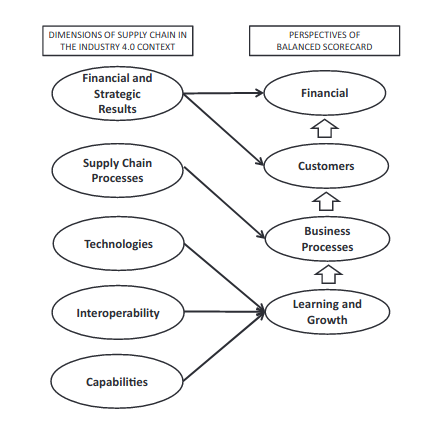
\includegraphics[width=0.8\textwidth,height=7cm]{Industry-4}
    \caption{Modifikasi BSC untuk kompleksitas Supply Chain di Era Industri 4.0}
    % \label{fig:my_image}
\end{figure}


\subsection*{Kesimpulan}
ttyyy

\bibliographystyle{apacite}
\bibliography{main}
\end{document}